
\begin{frame}

\begin{tcolorbox}
   \centering
   Backup Slides
\end{tcolorbox}

\end{frame}

\begin{frame}{Parameters}
Vacuum oscillations:
   $\sin^2\theta_v = 0.093$

Bipolar model animation:
\begin{itemize}
   \item $\theta_v = 0$
   \item $\alpha = 1$
   \item $\mu = 5$
\end{itemize}
Initial condition
\begin{itemize}
   \item \begin{equation*}
   \vec s = \begin{pmatrix}
      10^{-3} \\
      0 \\
      1
   \end{pmatrix}
   \end{equation*}
\end{itemize}

\end{frame}



%%%%%%%%%%%%%%%%%%%%%%%%%%%%%%%%%%%%%%%


\begin{frame}{Rabi Oscillations With Multiple Driving Frequencies}


\only<1>{
Consider Rabi oscillation with two driving frequencies $k_1=n_1 k$, $k_2=n_2 k$

\begin{equation*}
    \vec H = \begin{pmatrix}
    0\\
    0\\
    \omega_m
    \end{pmatrix} + \alpha_1\begin{pmatrix}
     \cos(k_1x)\\
    -\sin(k_1x)\\
    0
\end{pmatrix} + \colorbox{blue!50}{$\alpha_2\begin{pmatrix}
    \cos(k_2x)\\
    -\sin(k_2x)\\
    0
    \end{pmatrix}$}
\end{equation*}

Corotating frame of the second potential



\begin{equation*}
    \vec H = \begin{pmatrix}
    0\\
    0\\
    \omega_m - k_2
    \end{pmatrix} + \alpha_1\begin{pmatrix}
     \cos(k_1-k_2x)\\
    -\sin(k_1-k_2x)\\
    0
\end{pmatrix} + \colorbox{blue!50}{$\alpha_2\begin{pmatrix}
    1\\
    0\\
    0
    \end{pmatrix}$}
\end{equation*}

}

\only<1>{
Energy gap in this frame becomes the length of the vector

\begin{equation*}
    \begin{pmatrix}
    0\\
    0\\
    \omega_m - k_2
\end{pmatrix} + \colorbox{blue!50}{$\alpha_2\begin{pmatrix}
    1\\
    0\\
    0
    \end{pmatrix}$}
\end{equation*}
}

\only<2->{

% Energy gap in this frame becomes the length of the vector
% \begin{equation*}
% \sqrt{(\omega_{\mathrm m} - k_2)^2 + \alpha_2^2 } \to \omega_{\mathrm m} - k_2 + \frac{1}{2}\frac{\alpha_2^2}{\omega_{\mathrm m}-k_2}
% \end{equation*}

Relative detuning

\begin{equation*}
D' =  \left\vert \frac{\omega_{\mathrm m} - k_1 }{\alpha_1} + \frac{\alpha_2^2}{2\alpha_1(\omega_{\mathrm m}-k_2)} \right\vert
\end{equation*}

}

\end{frame}

\begin{frame}{Multiple Frequencies in Matter Potential}




\begin{equation*}
\lambda(x) = \lambda_0 + \sum_{a=1}^N A_a \sin(k_a x )
\end{equation*}


\begin{tcolorbox}[title=Hamiltonian in Rabi Basis]


\begin{equation*}
\mathbf{\widetilde H}= -\frac{\omega_{\mathrm m}}{2}\sigma_3 + \frac{1}{2} \sum_{n_1=-\infty}^\infty \cdots \sum_{n_N=-\infty}^\infty \begin{pmatrix}
0 &  B_{\{n_a\}} e^{i  {\color{red} \sum_a n_a k_a } x}\\
  B_{\{n_a\}}^* e^{ -i  {\color{red} \sum_a n_a k_a } x} & 0
\end{pmatrix}
\end{equation*}


where
\begin{align*}
    B_{\{n_a\}} &= -(-i)^{\sum_a n_a} \tan 2\theta_m \left( {\color{red}\sum_a n_a k_a} \right) \left( \prod_a J_{n_a}\left( \frac{A_a}{k_a}\cos 2\theta_m \right) \right)
    %\Phi_{\{n_a\}} &= e^{i\left( \sum_a n_a \phi_a \right)}.
\end{align*}




\end{tcolorbox}




\end{frame}




%%%%%%%%%%%%%%%%%%%%%%%%%%%%%%%%%%%%%%%%%%%%%%


\begin{frame}{MAA and MZA}

\begin{equation*}
   \tilde \epsilon = \frac{ v^\mu a_\mu }{ v^\alpha k_\alpha }
\end{equation*}


\end{frame}


\begin{frame}{Dispersion Relations}

Solve $k$ for MAA solutions
\begin{equation*}
   1 = \frac{1}{4k} \int \mathrm du G(u) \frac{ 1 - u^2 }{ \omega/k - u }.
\end{equation*}
around  $\omega\to 0$.

\pause

Apply Stokhotski-Plemelj theorem
\begin{align*}
\operatorname{Re}(k) =& \frac{1}{4}\left(  \mathcal{P} \int \mathrm d u G(u) \frac{ 1 - u^2 }{ - u }  \right)\label{eqn-re-k-arbitrary-spectrum} \\
\operatorname{Im}(k) =&  \frac{\pi}{4}G(0) \operatorname{Sign}\left( \omega \right) \operatorname{Sign}\left(  \operatorname{Im}(k)  \right).
\end{align*}

\pause

\begin{itemize}
   \item $G(0) \operatorname{Sign}(\omega) > 0$: $\lvert \operatorname{Im}(k) \rvert  =  \frac{\pi}{4}\lvert G(0)\rvert$
   \item $G(0) \operatorname{Sign}(\omega) < 0$: $\lvert \operatorname{Im}(k) \rvert  = 0$
\end{itemize}

\pause
\begin{tcolorbox}
   Gap between dispersion relation and $\omega=0$
\end{tcolorbox}


% \begin{frame}{Dispersion Relation}
% For MZA solutions
%
%
% \end{frame}


% \begin{align*}
% &\left(4\operatorname{Re}(k) - \mathcal P \int \frac{G(u)}{u} \mathrm d u + U_1 \right)^2  - \left( \operatorname{Sign}(\omega \operatorname{Im}(k) )\pi G(0) +4 \operatorname{Im}(k) \right)^2 \\
% =& - \left( \mathcal P \int \frac{G(u)}{u} \mathrm du + U_1 \right) \pi \operatorname{Sign}(\omega \operatorname{Im}(k) ) G(0),
% \end{align*}

% \begin{equation*}
%    \operatorname{Im}(k) = - \frac{1}{4} \pi G(0) \operatorname{Sign}(\omega \operatorname{Im}(k) ) \left(  1 \pm \frac{ \mathscr P \int \frac{G(u)}{u} du + \int G(u) u du }{ 4 \operatorname{Re}(k) - \mathscr P \int \frac{G(u)}{u} du + \int G(u) u du }  \right)
% \end{equation*}

\end{frame}

\begin{frame}{Dispersion Relations and Instabilities}


       \begin{textblock*}{100pt}(230pt,10pt)
           Remake of Fig.3 of Izaguirre et al, 2017
       \end{textblock*}

Define $u=\cos\theta$

Garching spectrum:

   \begin{figure}
      \minipage{0.49\textwidth}
        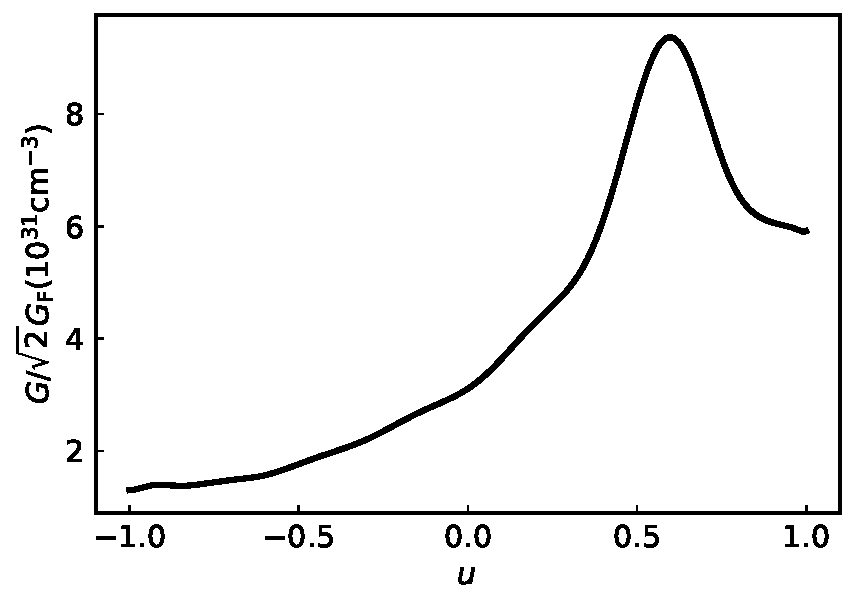
\includegraphics[width=\linewidth]{assets/dr/spectGarchingPlt.pdf}
        \caption*{Garching spectrum $G(u)$}
      \endminipage\hfill
      \minipage{0.49\textwidth}
      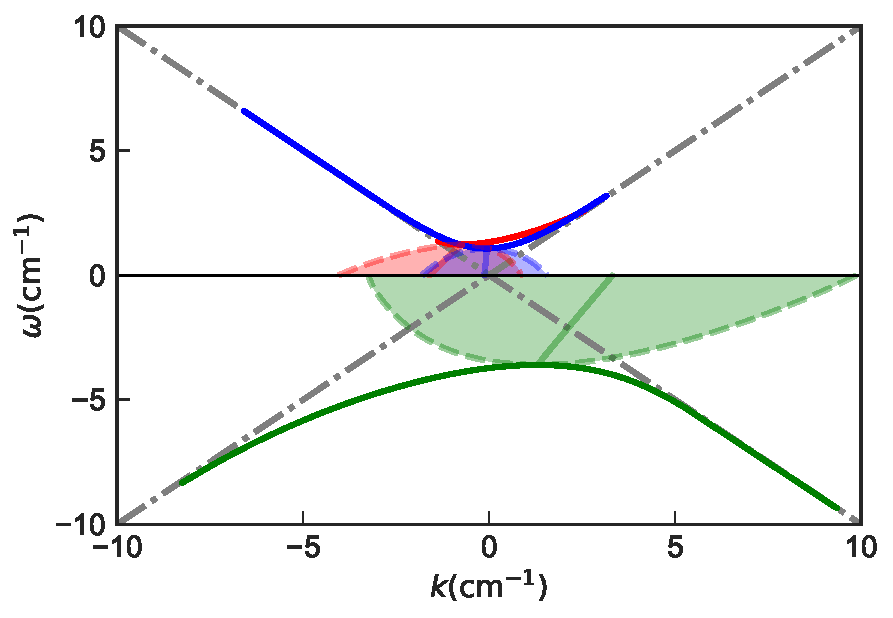
\includegraphics[width=\linewidth]{assets/dr/spectGarchingDRLSAPltBlob.pdf}
      \caption*{ MAA: red; MZA: blue and green }
      \endminipage\hfill
    %   \caption*{Dispersion relation and linear stability analysis (right panel) for a spectrum constructed from Garching 1D simulation data (left panel). Solid red line is dispersion relation for MAA solution while blue and green lines are for MZA solutions. Light red (blue and green) blob is instability for MAA (MZA) solution.
    %    }
   \end{figure}

\pause
\begin{tcolorbox}
   \begin{itemize}
      \item
      \color{black}MAA solutions: unstable region stops at $\omega\to 0$
      \item
      \color{black} MZA solutions: instabilities are different for region $\omega>0$ and $\omega<0$.
   \end{itemize}
\end{tcolorbox}
\pause
\begin{tcolorbox}
   \color{black} Instabilities might occur in gaps of DR and $\omega=0$ if there is any.
\end{tcolorbox}

\end{frame}




%%%%%%%%%%%%%%%%%%%%%%%%%%%%%%
%%%% Neutrino Halo Problem






\begin{frame}{Neutrino Halo}

\only<1>{
\begin{figure}
   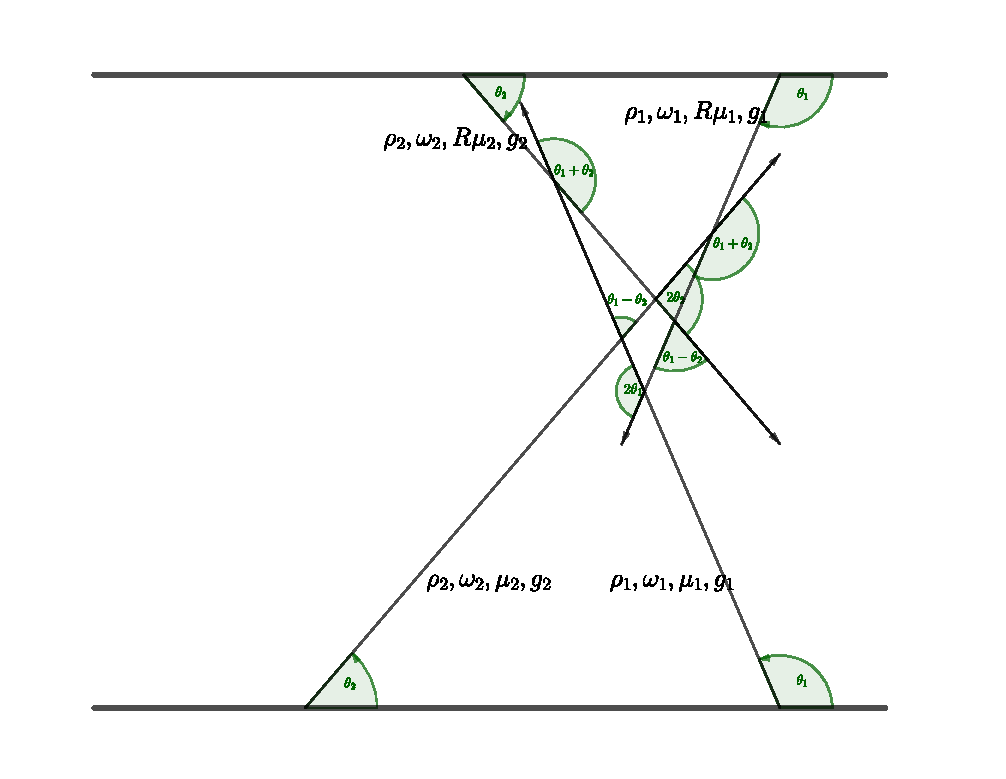
\includegraphics[width=\textwidth]{assets/halo-line-model}
\end{figure}
}

\only<2>{

\begin{columns}[T]
   \begin{column}{0.5\textwidth}
      Assumptions
      \begin{itemize}
         \item Neutrinos are translational symmetric on the emission line.
         \item Reflection obays Snell's law.
         \item Neutrinos are reflected on a fixed surface $z=L$.
         \item Neutrino reflections are translational symmetric.
      \end{itemize}

   \end{column}

   \begin{column}{0.5\textwidth}
      \begin{figure}
         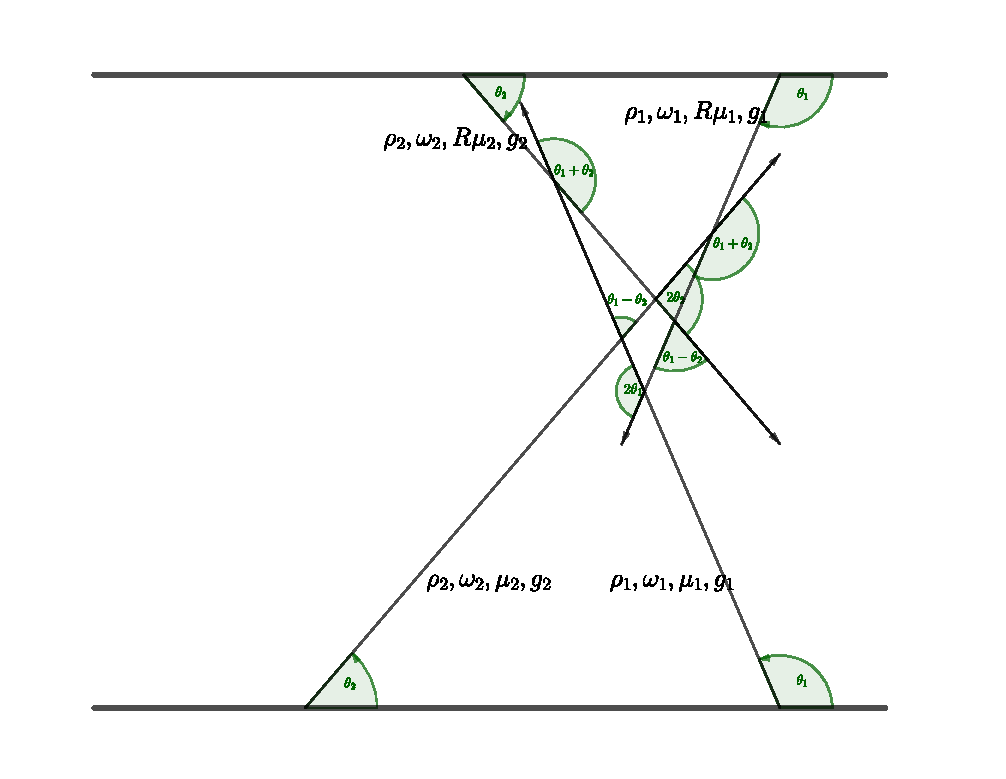
\includegraphics[width=\textwidth]{assets/halo-line-model}
      \end{figure}
   \end{column}
\end{columns}


}

\end{frame}

\subsection{Flavor Isospin Picture}

\begin{frame}{Flavor Isospin}


\begin{figure}
   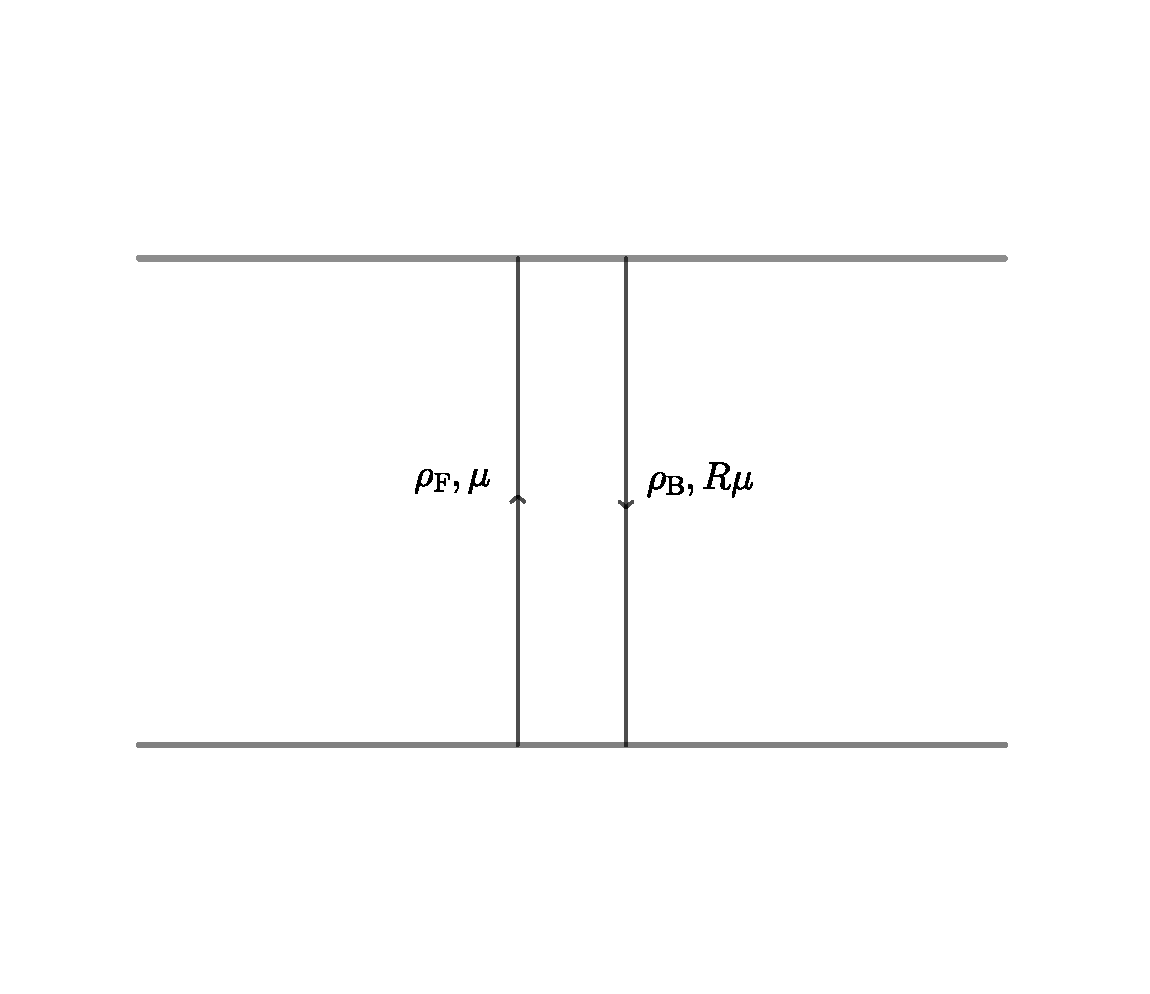
\includegraphics[width=\textwidth]{assets/halo-line-model-single-beam}
\end{figure}


\end{frame}



\begin{frame}{Relaxation Scheme}

\begin{tcolorbox}[title=Algorithm,standard jigsaw,
    opacityback=0]
   \begin{enumerate}
      \item Calculate forward beam using null backward beam;
      \item Calculate backward beam using forward beam calculated in step 1;
      \item Calculate forward beam using backward beam calculated in step 2;
      \item Repeat 2 and 3 until the beams reach equilibrium.
   \end{enumerate}
\end{tcolorbox}




\end{frame}




\begin{frame}{Numerical Method}

\begin{tcolorbox}
\begin{figure}
   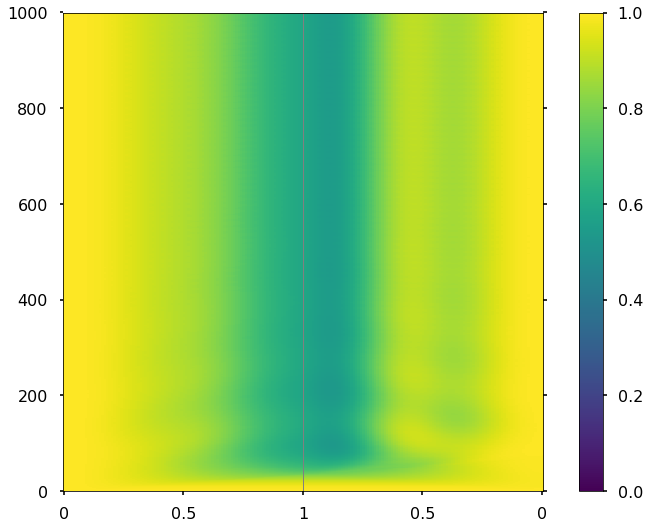
\includegraphics[width=0.9\textwidth]{assets/relax-color}
   \caption*{\color{black}Horizontal axis is the location of neutrinos; Vertical axis is the number of iteration steps; Color indicates the electron flavor probability.}
\end{figure}
\end{tcolorbox}

\end{frame}


\begin{frame}{Numerical Method}

\begin{tcolorbox}
   \begin{figure}
      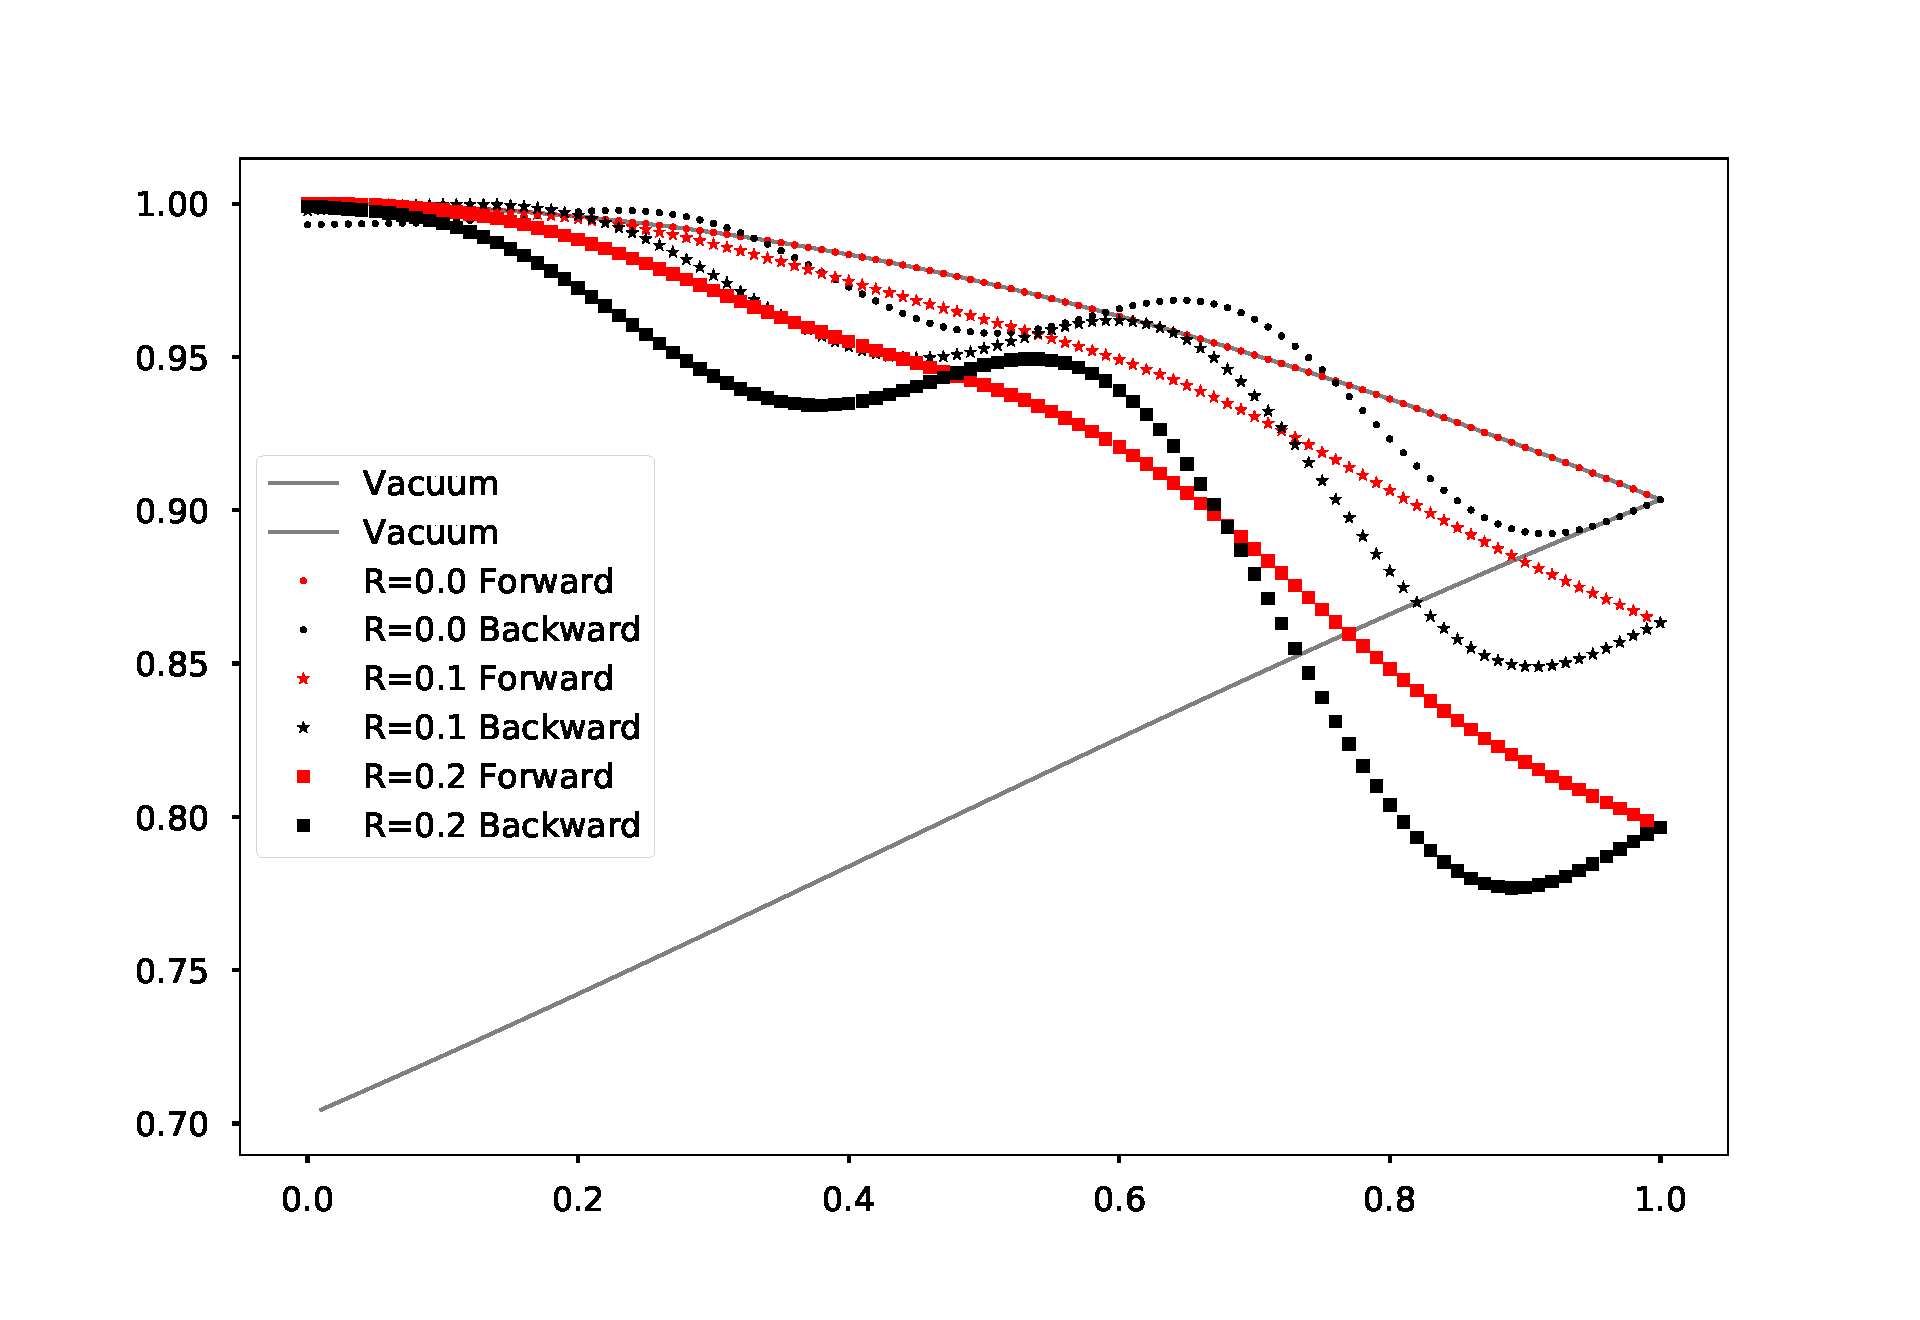
\includegraphics[width=\textwidth]{assets/halo-mu-4-r-multiple}
   \end{figure}
\end{tcolorbox}

\end{frame}

\begin{frame}{Linear Stability Analysis}

EoM

   \begin{align*}
    i \partial_t \vec s_F &= \mathbf s_F \times (\vec {H}_v +R \mu \vec s_B) \\
      i\partial_t \vec s_B &= \vec s_B \times (- \vec H_v - \mu \vec s_F) .
   \end{align*}

Compare with bipolar

\begin{align*}
    i\partial_t \vec s &= \mathbf s \times ( \eta \vec H_v + \alpha \mu \bar{\vec s} )\\
    i\partial_t \bar{\vec s} &= \bar{\vec s} \times ( \eta \vec H_v + \mu \vec s )
\end{align*}


\end{frame}


\begin{frame}{Linear Stability Analysis}


\begin{tcolorbox}

   % \only<1>{
      \begin{figure}
         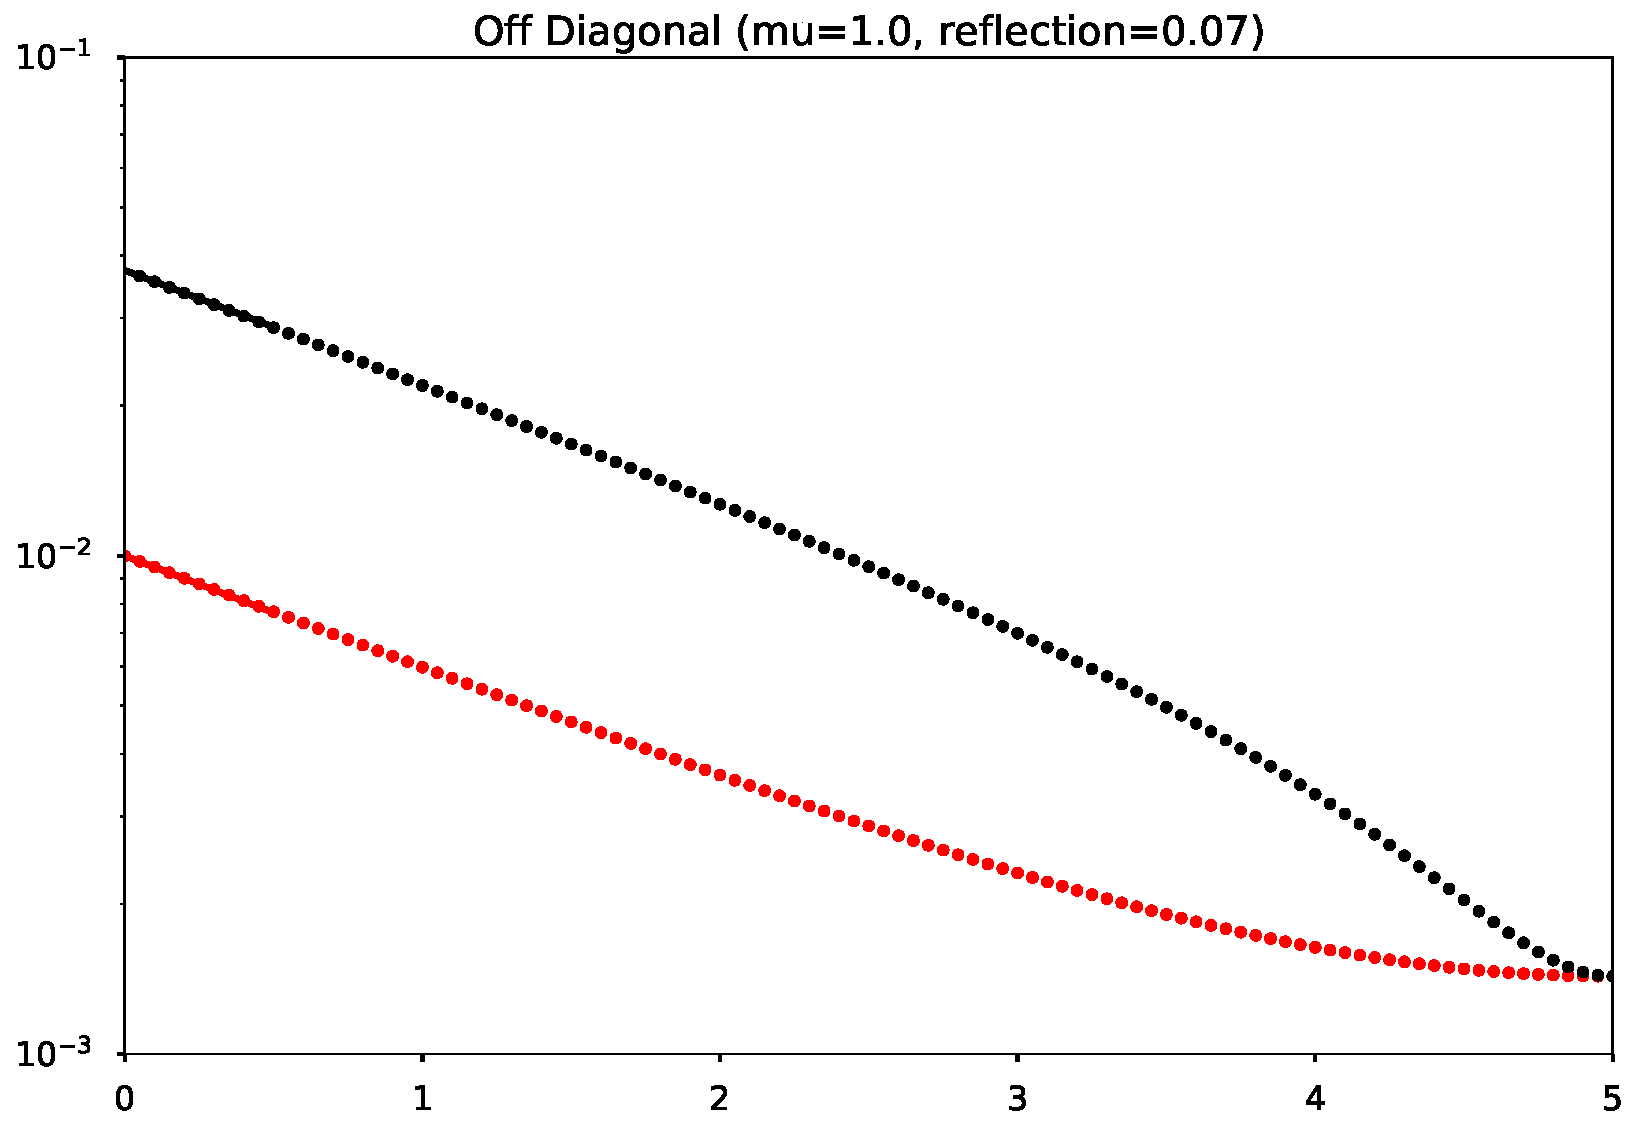
\includegraphics[width=\textwidth]{assets/halo-mu-1-reflection-0p07}
      \end{figure}
      % }

   % \only<2>{
   %    \begin{figure}
   %       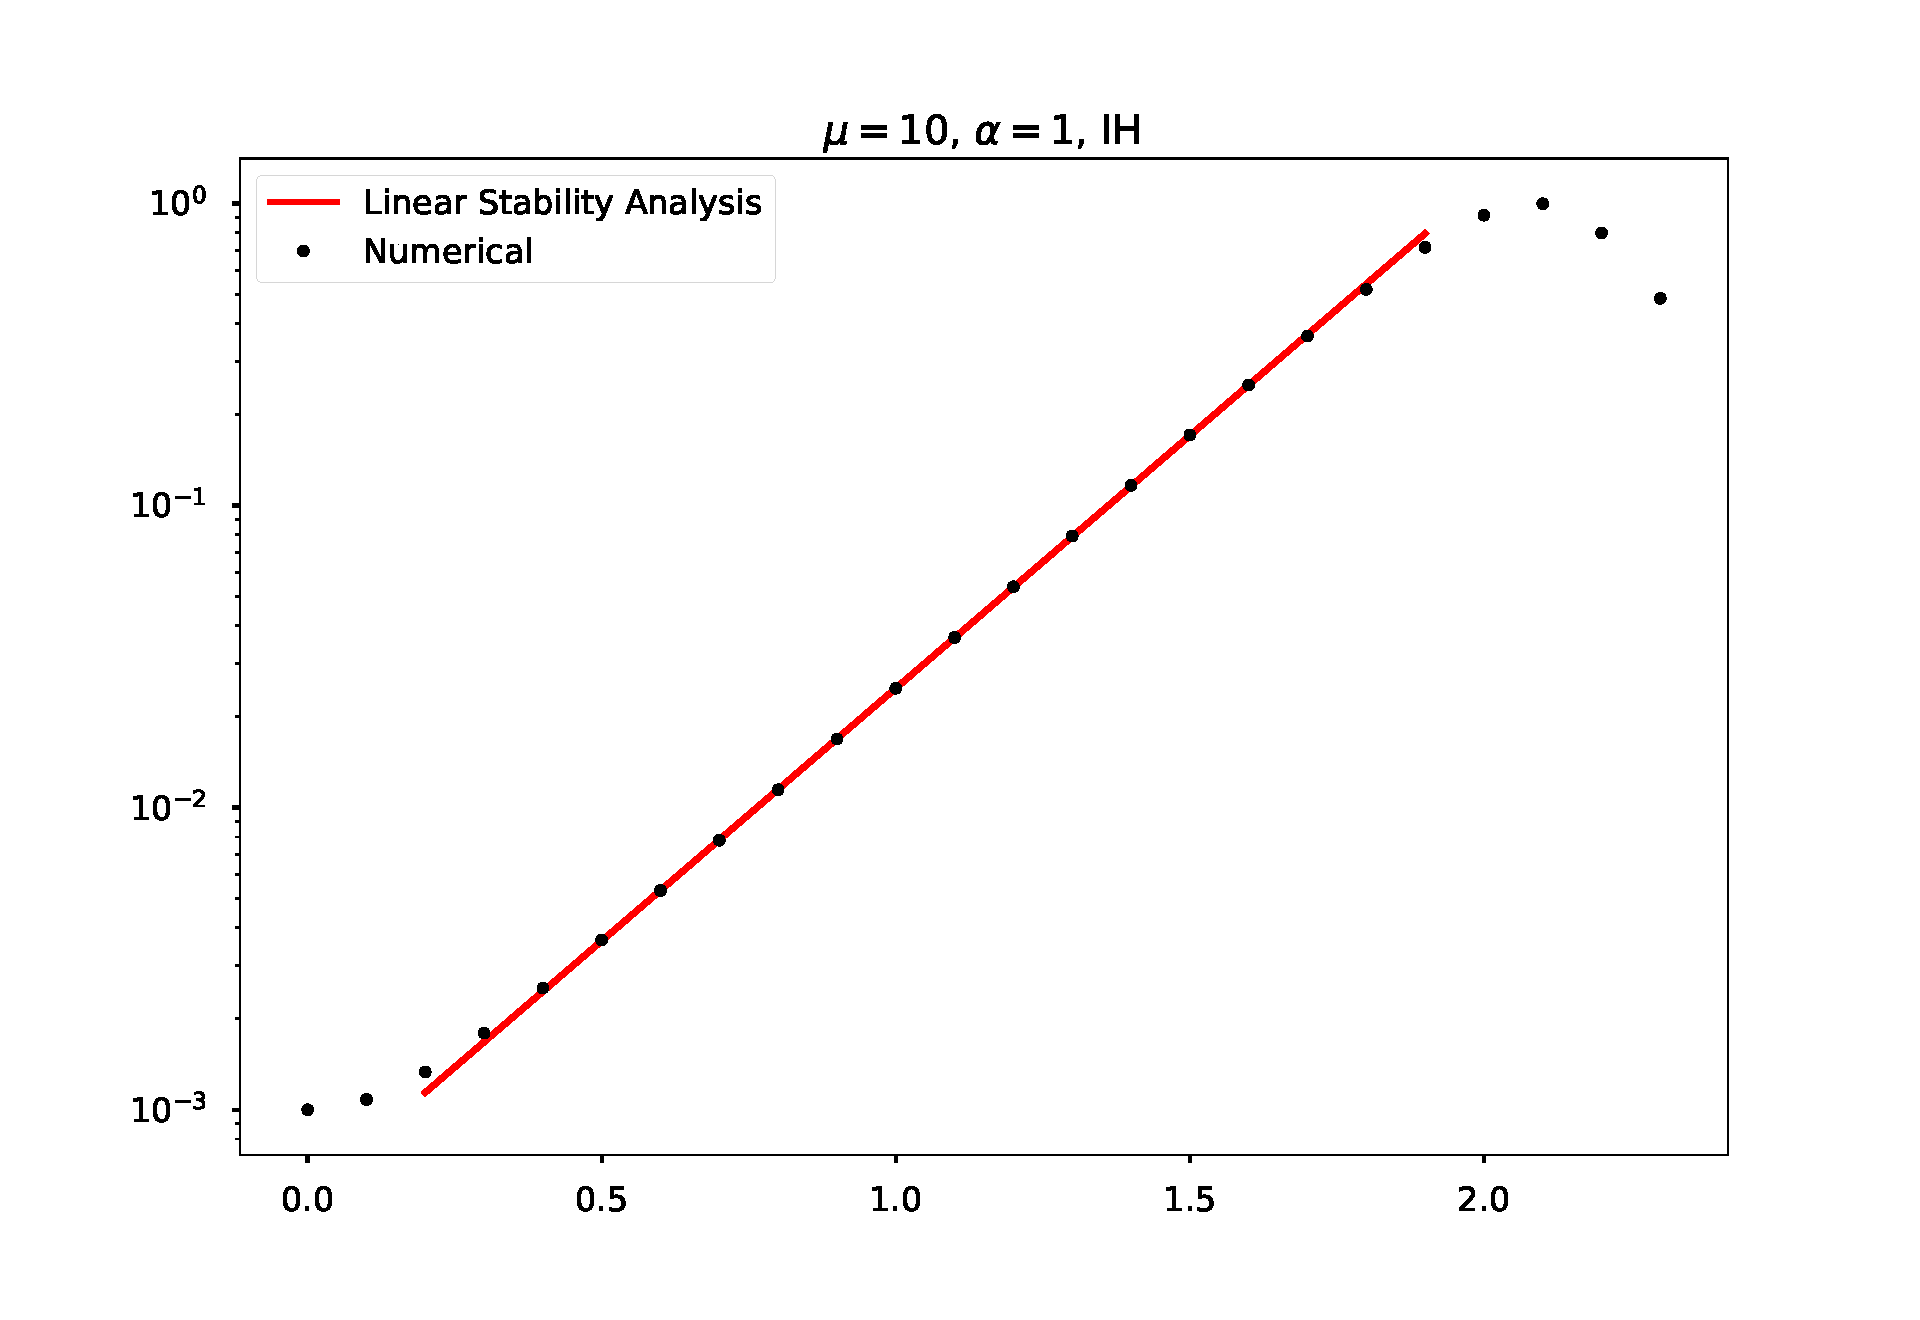
\includegraphics[width=\textwidth]{assets/halo-mu-4-compare-bipolar}
   %    \end{figure}
   % }

\end{tcolorbox}



\end{frame}
